%%%%%%%%%%%%%%%%%%%%%%%%%%%%%%%%%%%%%%%%%%%%%%%%%%%%%%%%%%%%%%%%%%%%%%%%%%%%%%%
%2345678901234567890123456789012345678901234567890123456789012345678901234567890
%        1         2         3         4         5         6         7         8

\documentclass[journal]{IEEEtran}  % Comment this line out
                                                          % if you need a4paper
%\documentclass[a4paper, 10pt, conference]{ieeeconf}      % Use this line for a4
                                                          % paper

\IEEEoverridecommandlockouts                              % This command is only
                                                          % needed if you want to
                                                          % use the \thanks command
%\overrideIEEEmargins
%\bibliographystyle{IEEEtran}
%\bibliography{IEEEabrv,bibliography}
% See the \addtolength command later in the file to balance the column lengths
% on the last page of the document
% The following packages can be found on http:\\www.ctan.org
%\usepackage{graphics} % for pdf, bitmapped graphics files
\usepackage{graphicx}
\usepackage{placeins}
\usepackage{caption}
\usepackage{float}
%\usepackage[backend=bibtex,style=verbose-trad2]{biblatex}
%\usepackage{epsfig} % for postscript graphics files
%\usepackage{mathptmx} % assumes new font selection scheme installed
%\usepackage{times} % assumes new font selection scheme installed
%\usepackage{amsmath} % assumes amsmath package installed
%\usepackage{amssymb}  % assumes amsmath package installed

\title{
	Monitoring of biodegradation process using an embedded system to report data to a smartphone
}

\author{
	Gonzalez O. and Ramirez R.% <-this % stops a space
}


\begin{document}



\maketitle
\thispagestyle{empty}
\pagestyle{empty}


%%%%%%%%%%%%%%%%%%%%%%%%%%%%%%%%%%%%%%%%%%%%%%%%%%%%%%%%%%%%%%%%%%%%%%%%%%%%%%%%
\begin{abstract}

In this paper, it is presented an approach to monitor biodegradation process physical variables using an embedded system. The system is capable of measuring temperature and light and will estimate other important variables such as the biomass concentration and dissolved oxygen. This system will be able to control desired variables using embedded control scheme and report its results to Matlab in order to plot and to a smartphone and notify the biotechnologist important changes during the biodegradation process.

\end{abstract}


%%%%%%%%%%%%%%%%%%%%%%%%%%%%%%%%%%%%%%%%%%%%%%%%%%%%%%%%%%%%%%%%%%%%%%%%%%%%%%%%
\section{INTRODUCTION}
Nowadays, the biodegradation process monitoring and control of physical measured values represent a challenge for biotechnologists since the classic way to do it involves doing it by themselves, i.e. supervising if the results processes are going well by eyesight. Light, color, temperature, levels of oxygen, volume are examples of signals desired to control in order to complete a biorreaction experiment. Nonetheless the control scheme does not always end well and the biotechnologist in charge of the experiment must be around in case anything comes up. The embedded systems have shown a good workaround to process input signals due to their powerful capabilities in terms of memory, speed, power consumption, IoT, communication protocols.
The document is outlined as follows: In the next section an overview of the system structured as a block diagram as well as a description of each block and its function, next it will be presented the classic approach for virtual sensors and the algorithms solving the control scheme satisfying the set points requirements. Finally important graphs are shown and conlcusions close this work.

\section{MATHEMATICAL FORMULATION}
The system's mathematical model is a description providing information of physical variables. In this article it is described the mathematical model of a biorreactor in which a total of four variables are of interest:

\begin{itemize}
	\item Dissolved oxygen
	\item Biomass concentration
	\item Organic matter degradation
	\item Volume
\end{itemize}

The next model describes the degradation process of organic matter ($S_c$), concentration of dissolved oxygen ($S_{O_{t}}$), volume ($V_{t}$) and biomass concentration ($X_t$):
\begin{equation}
{
	\begin{array}{cc}
	\frac{dX_{t}}{dt}=\mu X_{t} - \frac{q_{in}}{V}X_{t} \\
	\frac{dS_{c}}{dt}=-k_{1}\mu X_{t} - \frac{q_{in}}{V}(S_{c,in}-S_{c}) \\
	\frac{dS_{O_{t}}}{dt}=-k_{2}\mu X_{t} - b X_{t}\frac{q_{in}}{V}(S_{c,in}-S_{O_{t}})-K_{L}\alpha(S_{os}-S_{O_{t}}) \\
	\frac{dV_{t}}{dt}=q_{in}
	\end{array}}
\end{equation}

where $\mu=0.1916 h^{-1}$ is the specific growth rate of the
biomass concentration, $k_1=3.7 L^{-1}$ is the coefficient that determines the transformation between the biomass $X_{t}$ and the organic matter $S_{c}$, $k_2=1 L^{-1}$ is the transformation coefficient between $X_{t}$ and $S_{O_{t}}$, $b=0.0004 mgO_{2}/mg$ is the endogenous respiration kinetic constant, $k_{L}\alpha=0.1 s^{-1}$ is the transfer coefficient for the oxygen saturation concentration and finally $q_in$ ($ml/L$) is the inlet flow rate.
The mathematical model sometimes in real applications are not possible since the sensors might be too expensive to include it in an economic system or it takes hours to get precise sensor characterization, a solution to this is the "state estimation process" in which it is build an aritifial copy of the system reproducing the original's behavior of the system.


\section{SYSTEM BLOCK DIAGRAM}

The system block diagram Figure \ref{fig:figure1} shows a general workaround solving the problem, the embedded system is based on a Intel Edison microprocessor with Linux as operating system. This development was chosen because the development environment and IoT capabilities. The input is defined as two sensors providing temperature and light readings in analog format, these sensors already have a coupling stage to make possible a straightforward connection between the sensors and microprocessor. Next, we have the microprocessor stage with Bluetooth and WiFi modules, this stage is capable of performing fast operations then, it's totally possible to code a PID algorithm, input signals handling and output signals. Finally the system will provide information to the user via Bluetooth, sending notifications whenever a sensor is above the user-defined setpoint.

\begin{figure}[h]
	\centering
	\captionsetup{justification=centering}
	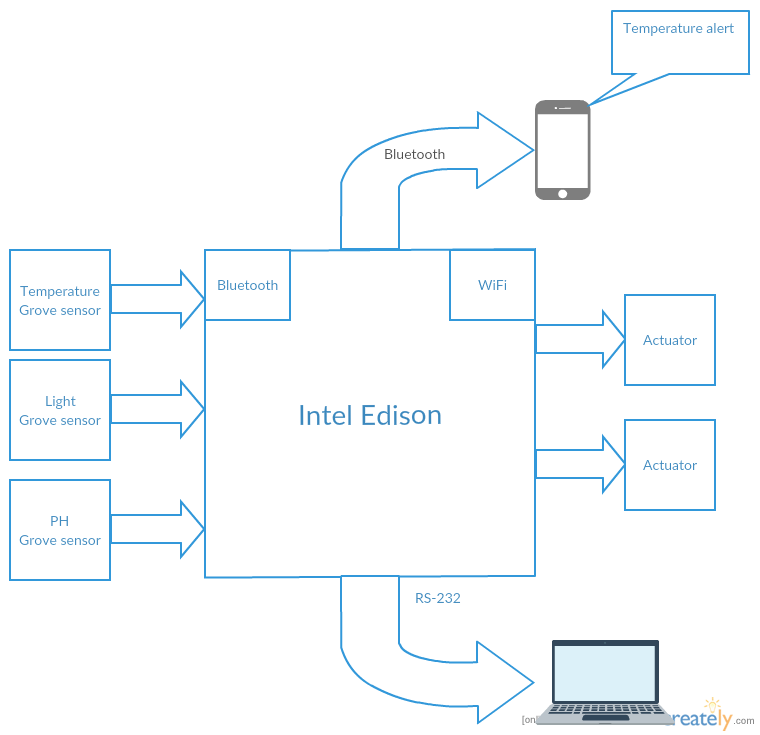
\includegraphics[width=3in]{Embedded_bio.png}
	\caption{Embedded system.}
	\label{fig:figure1}
\end{figure}

\section{SENSORS CHARACTERIZATION}
The following sensors were measured:
	\begin{itemize}
		\item Light
		\item Temperature
		\item PH
	\end{itemize}

These variables have to be controlled and monitored in a biorreaction process to assure that the biological environment will remain active. To achieve a valid criteria of physical values measured from the sensors, there will be a graphic response of the physical value provided by the sensor and the desired physical value relationship.

\begin{figure}
	\centering
	\captionsetup{justification=centering}
	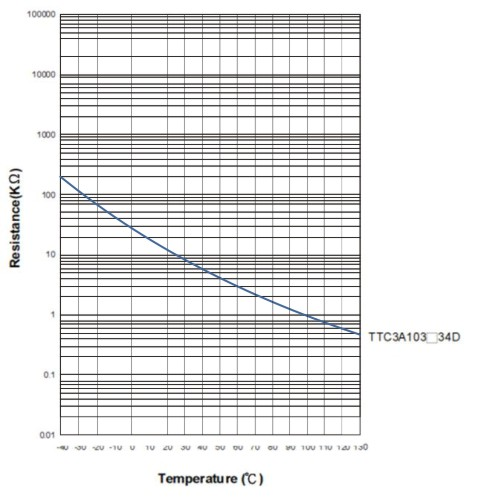
\includegraphics[width=3in]{temp.jpg}
	\caption{Temperature characterization.}
	\label{fig:figure2}
\end{figure}

\section{ALGORITHM AND DESIGN}
The system's algorithm to solve the problem is based on a state machine handling states related to processing stages of the system. 

\begin{figure}
	\centering
	\captionsetup{justification=centering}
	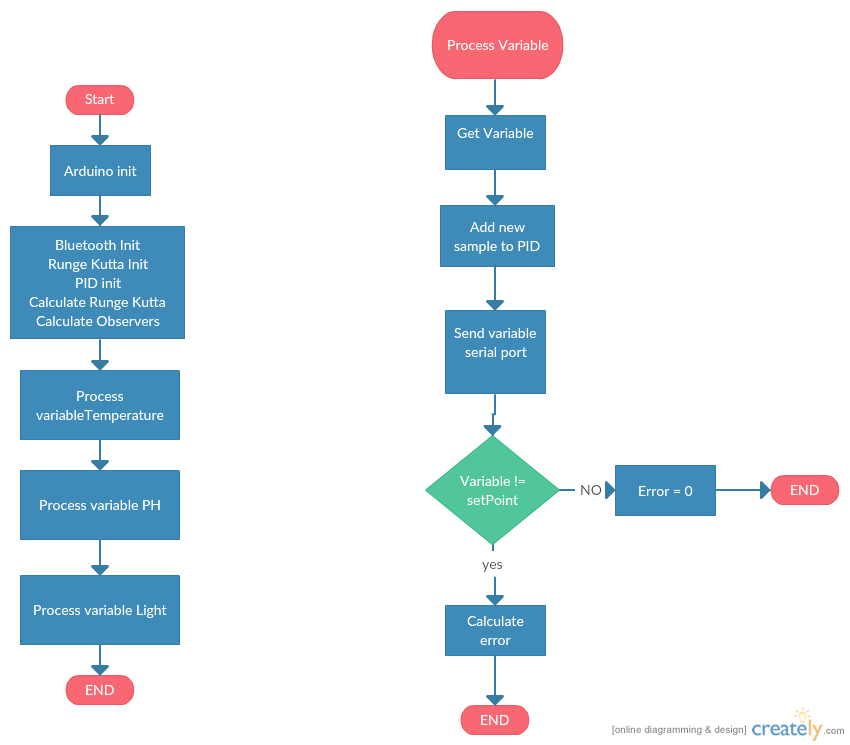
\includegraphics[width=3in]{flowchart.png}
	\caption{Flow diagram.}
	\label{fig:figure4}
\end{figure}

\section{RESULTS AND GRAPHICS}
\begin{figure}
	\centering
	\captionsetup{justification=centering}
	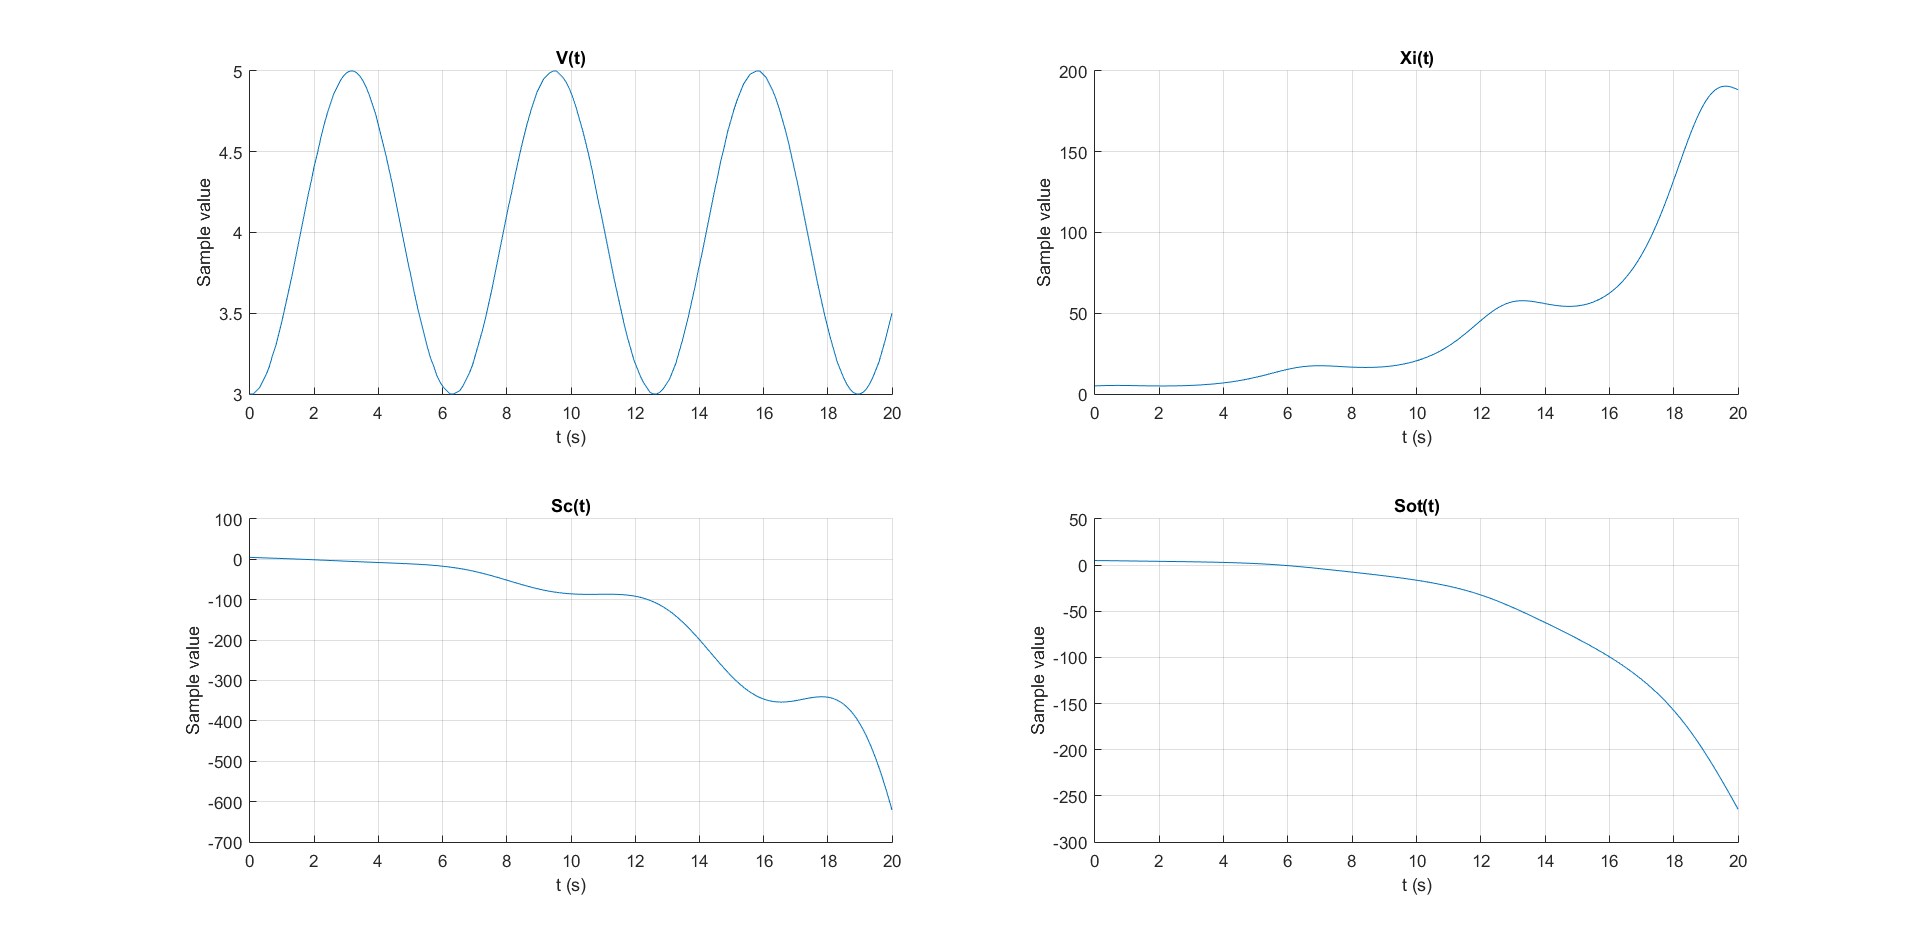
\includegraphics[width=3in]{matlab.png}
	\caption{Matlab figures simulation}
	\label{fig:figure5}
\end{figure}


\section{CONCLUSIONS}
The embedded systems \cite{IEEEexample:article_typical} have shown strong cabilities for matrix processing and its speed solving problems. Any mathematical model can be modeled in a embedded system, however having all variables in an equation is not always the best option for a specific hardware. The use of observers ease the mathematical model approximating variables not described in the model by using the ones in the mathematical model. Set point calibration is an important step in these types of system in which the environment must remain as constant as possible to establish a set point reference. Biodegradation process mathematical model can be described as precise as possible but it's always recommended to assess the impact of having robust mathematical models or training observer to accomplish the system's goal.


%\addtolength{\textheight}{-12cm}   % This command serves to balance the column lengths
                                  % on the last page of the document manually. It shortens
                                  % the textheight of the last page by a suitable amount.
                                  % This command does not take effect until the next page
                                  % so it should come on the page before the last. Make
                                  % sure that you do not shorten the textheight too much.

%%%%%%%%%%%%%%%%%%%%%%%%%%%%%%%%%%%%%%%%%%%%%%%%%%%%%%%%%%%%%%%%%%%%%%%%%%%%%%%%



%%%%%%%%%%%%%%%%%%%%%%%%%%%%%%%%%%%%%%%%%%%%%%%%%%%%%%%%%%%%%%%%%%%%%%%%%%%%%%%%



%%%%%%%%%%%%%%%%%%%%%%%%%%%%%%%%%%%%%%%%%%%%%%%%%%%%%%%%%%%%%%%%%%%%%%%%%%%%%%%%

\bibliography{bibliography}
\bibliographystyle{IEEEtran}


\end{document}